\documentclass[a4paper,11pt]{article}
\usepackage[utf8]{inputenc}
\usepackage[usenames,dvipsnames]{color}
\usepackage{graphicx}
\usepackage[justification=centering,labelfont=bf]{caption}
\usepackage{listings}
\usepackage{csvsimple}
\usepackage{booktabs,mathptmx,siunitx}
\lstset{ % For diff
  basicstyle={\footnotesize\ttfamily},
  breakatwhitespace=false,
  breaklines=true,
  language=C,
  frame=single,
  captionpos=b,
  extendedchars=true,
  showspaces=false,
  showstringspaces=false,
  escapeinside=||,
  showtabs=false,
  tabsize=8,
  moredelim=**[is][\color{OliveGreen}]{@}{@},
}

\newcommand{\blueline}[1]{\textcolor{blue}{#1}}

\newcommand{\assignatura}{Parallelism}
\newcommand{\titol}{First Deliverable}

\newcommand{\Pautor}{Héctor Ramón Jiménez}
\newcommand{\Sautor}{Alvaro Espuña Buxó}

\newcommand{\HRule}{\rule{\linewidth}{0.5mm}}

\newcounter{ProblemCounter}
\newcommand{\question}{%
  \setcounter{enumi}{\value{ProblemCounter}}%
  \stepcounter{ProblemCounter}%
}
\newcommand{\answer}[1]{
  {\bf {#1}}
}

\begin{document}

\begin{titlepage}
  \begin{center}
    \textsc{\Large \assignatura}\\[1.5cm]
    \HRule \\[0.4cm]
     { \huge \bfseries \titol \\[0.4cm] }
    \HRule \\[2.5cm]
    \begin{minipage}{0.4\textwidth}
      \begin{flushleft}
        \large \Pautor
      \end{flushleft}
    \end{minipage}
    \begin{minipage}{0.4\textwidth}
      \begin{flushright}
        \large \Sautor
      \end{flushright}
    \end{minipage}

    \vfill
    {\large \today}
  \end{center}
\end{titlepage}

\section*{Node architecture and memory}
\begin{enumerate}
  \question \item Describe (better if you do a simple drawing) the
  architecture of the computer in which you are doing this lab session
  (number of sockets, cores per socket, threads per core, cache
  hierarchy size and sharing, and amount of main memory).
\end{enumerate}

\section*{Timing sequential and parallel executions}
\begin{enumerate}
  \question \item Indicate the library header where the structure
  struct timeval is declared and which are its fields.

  \answer{
    It is defined in \texttt{sys/time.h}. Its fields are:
    \begin{itemize}
      \item tv\_sec: Time in seconds
      \item tv\_usec: Time in microseconds
    \end{itemize}
  }

  \question \item Plot the execution time when varying the number of
  threads for {\tt pi\_omp.c}. Reason about how the number of threads
  influence on the execution time.

  \begin{figure}[h!]
    \begin{center}
    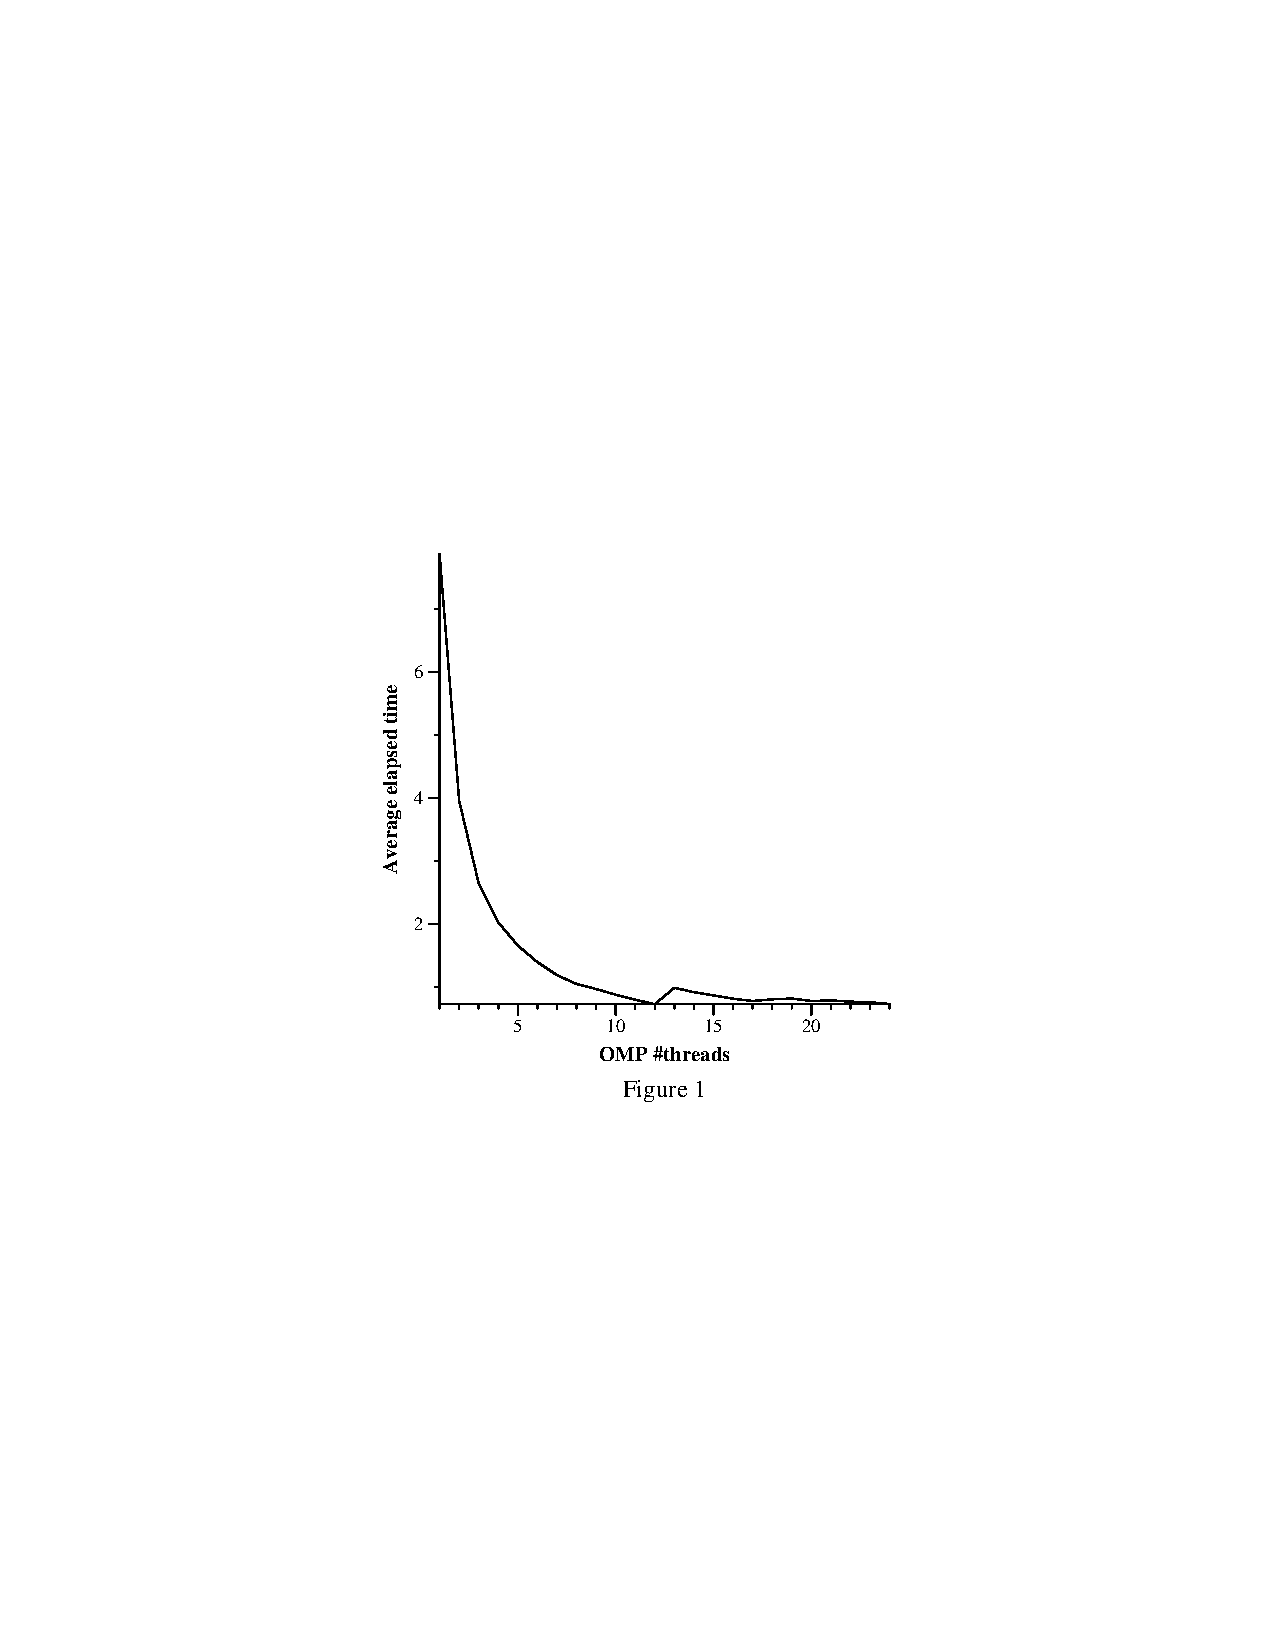
\includegraphics[trim=150 250 150 250, clip, width=0.7\textwidth]{pi_omp/threads.pdf}
    \caption{Figure showing execution time as function of the
      number of threads used}
    \end{center}
  \end{figure}

  \answer{
    When using from 1 to 12 threads the execution time follows the formula $\frac{execution\:time\:with\:1\:thread}{number\:of\:threads}$, as expected.

    When more than 12 threads are used there is a slight overhead. This
    was expected too because, despite that each node supports 2 threads
    per core, the threads are sharing resources.
  }

\end{enumerate}

\section*{Tracing parallel executions}
\begin{enumerate}
  \question \item From the two instrumented {\tt OpenMP} versions
  ({\tt pi\_omp\_sum\_local.c} and {\tt pi\_omp\_critical.c}), show a
  profile of the \% of time spent in the different {\tt OpenMP}
  states. Reason about the differences observed and guess which is the
  construct in the source code that is the cause of these differences.

  \begin{center}
  \begin{tabular}{| l || S | S |}
    \cline{2-3}
    \multicolumn{1}{l ||}{} & \multicolumn{1}{c |}{critical} & \multicolumn{1}{c |}{sum\_local} \\
    \hline\hline
    Running & 9.79 & 85.12 \\
    \hline
    Not created & 0.01 & 5.40 \\
    \hline
    Synchronization & 87.15 & 5.94 \\
    \hline
    Scheduling and Fork/Join & 0.26 & 7.89 \\
    \hline
    I/O & 3.01 & 2.55 \\
    \hline
  \end{tabular}
  \end{center}

  \answer{
    The differences are caused by the moment where the mutual exclusions are performed:
    \begin{itemize}
      \item The ``critical'' version performs mutual exclusions in each iteration. Therefore, every thread needs to be synchronized with all the other threads before performing an iteration!
      \item The ``sum\_local'' version only performs $num\_threads$ exclusions to reduce the local sums of each thread. Thus, this version can perform the most part of the computation without any synchronization with the other threads.
    \end{itemize}

  }

  \question \item For the two {\tt OpenMP} versions provided, fill in the
  following table with the time elapsed in each part of the code and
  the total elapsed time of the instrumented code (using 8 threads).

  \begin{center}
    \begin{tabular}{| l || S | S | S | S |}
      \cline{2-5}
      \multicolumn{1}{l ||}{} & \multicolumn{1}{c |}{REST\_MAIN} & \multicolumn{1}{c |}{PI\_COMPUTATION} & \multicolumn{1}{c |}{TIMING} & \multicolumn{1}{c |}{Total}\\
      \hline\hline
      critical & 5540.00 & 101118642.50 & 24749.00 & 132382580.88 \\
      \hline
      sum\_local & 5268.00 & 190077.88 & 16061.00 & 3767231.88 \\
      \hline
      \hline
      \textbf{SPEEDUP} & 1.05 & 531.98 & 1.54 & 35.14 \\
      \hline
    \end{tabular}
  \end{center}

  \answer{It is clear that the PI\_COMPUTATION has been performed faster in the sum\_local version, avoiding the synchronization in each iteration and obtaining a huge speedup.}
\end{enumerate}

\section*{Visualizing the task graph and data dependences}

\begin{enumerate}
  \question \item Include the source code for function {\tt dot\_product}
  in which you show the instrumentation that has been added in order
  to identify tasks and filter the analysis of variable(s) that cause
  the dependence(s).

  \answer{See attached file: \texttt{dot\_product.c}}

  \question \item Capture the task dependence graph and execution
  timeline (for 8 processors) for that task decomposition.

  \begin{figure}[h!]
    \begin{center}
    \includegraphics[width=1\textwidth]{dot_product/dependency_graph.pdf}
    \caption{Figure showing the entire task dependency graph of \texttt{dot\_product.c}}
    \end{center}
  \end{figure}
  
  \begin{figure}[h!]
    \begin{center}
    \includegraphics[trim=3300 0 3300 600, clip,width=1\textwidth]{dot_product/dependency_graph.pdf}
    \caption{Figure zooming the center section of the task dependency graph of \texttt{dot\_product.c}}
    \end{center}
  \end{figure}

  \begin{figure}[h!]
    \begin{center}
    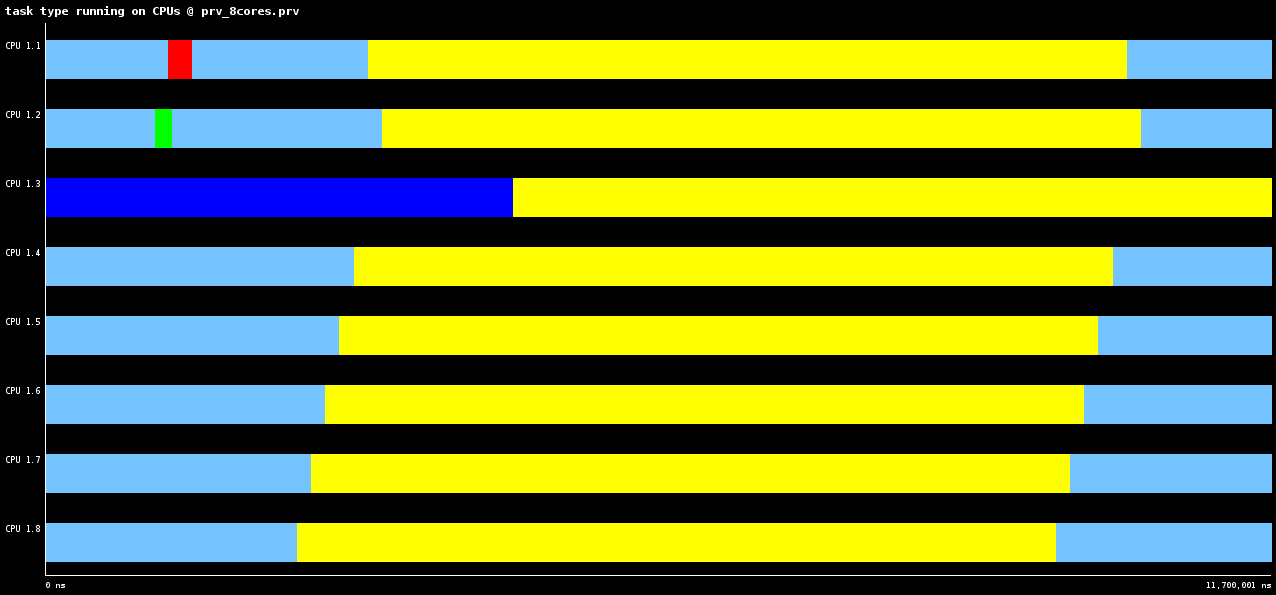
\includegraphics[width=1\textwidth]{dot_product/execution_graph_8_cores.png}
    \caption{Figure showing the execution timeline of \texttt{dot\_product.c} with 8 processors}
    \end{center}
  \end{figure}
\end{enumerate}

\section*{Analysis of task decomposition}
\begin{enumerate}
  \question \item Complete the following table for the initial and
  different versions generated for {\tt 3dfft\_seq.c}.

  \begin{center}
    \begin{tabular}{| c || c | c | c |}
      \hline
          {\bf Version} & $T_1$ & $T_{\infty}$ & {\bf Parallelism} \\
          \hline
          \hline
          sqe & & & \\
          \hline
          v1 & & & \\
          \hline
          v2 & & & \\
          \hline
          v3 & & & \\
          \hline
          v4 & & & \\
          \hline
    \end{tabular}
  \end{center}

  \question \item  With the results from the parallel simulation with
  2, 4, 8, 16 and 32 processors, draw the execution time and speedup
  plots for version {\tt v4} with respect to the sequential execution (that
  you can estimate from the simulation of the initial task
  decomposition that we provided in {\tt 3dfft\_seq.c}, using just 1
  processor).
\end{enumerate}

\end{document}
